\documentclass[aspectratio=169,11pt]{beamer}
\usepackage[utf8]{inputenc}
\usepackage[T1]{fontenc}
\usepackage[english]{babel}
\usepackage{amsmath,amssymb,booktabs,graphicx,listings,xcolor}
\usepackage{hyperref}

\definecolor{navy}{RGB}{20,45,74}
\definecolor{blue}{RGB}{31,105,140}
\definecolor{amber}{RGB}{190,116,32}
\definecolor{pale}{RGB}{241,245,248}
\definecolor{codebg}{RGB}{247,248,250}
\definecolor{codegreen}{RGB}{31,110,70}

\usetheme{default}
\setbeamercolor{normal text}{fg=navy,bg=white}
\setbeamercolor{structure}{fg=blue}
\setbeamercolor{frametitle}{fg=white,bg=navy}
\setbeamercolor{title}{fg=navy}
\setbeamercolor{block title}{fg=white,bg=blue}
\setbeamercolor{block body}{fg=navy,bg=pale}
\setbeamercolor{alerted text}{fg=amber}
\setbeamertemplate{navigation symbols}{}
\setbeamertemplate{footline}{%
  \leavevmode\hbox{%
    \begin{beamercolorbox}[wd=.88\paperwidth,ht=2.6ex,dp=1.1ex,leftskip=1em]{author in head/foot}%
      \scriptsize Acemoglu and Restrepo (2018) \hfill Lean formalization
    \end{beamercolorbox}%
    \begin{beamercolorbox}[wd=.12\paperwidth,ht=2.6ex,dp=1.1ex,center]{date in head/foot}%
      \scriptsize \insertframenumber/\inserttotalframenumber
    \end{beamercolorbox}}}
\setbeamerfont{frametitle}{size=\Large,series=\bfseries}
\setbeamerfont{title}{size=\LARGE,series=\bfseries}
\setbeamersize{text margin left=0.65cm,text margin right=0.65cm}

\lstdefinestyle{lean}{
  language={},
  basicstyle=\ttfamily\scriptsize,
  keywordstyle=\color{blue}\bfseries,
  commentstyle=\color{codegreen},
  backgroundcolor=\color{codebg},
  frame=single,
  rulecolor=\color{navy!25},
  columns=fullflexible,
  keepspaces=true,
  showstringspaces=false,
  breaklines=true,
  xleftmargin=0.25em,
  xrightmargin=0.25em
}

\newcommand{\source}[1]{\vfill{\tiny\color{navy!70}Source: #1}}

\title{The Race between Man and Machine}
\subtitle{Economic results, numerical checks, and a partial Lean formalization}
\author{fgalarzac}
\date{Repository 6 \textperiodcentered{} September 2026}

\begin{document}

\begin{frame}[plain]
  \titlepage
  \begin{center}
    \small\href{https://github.com/fgalarzac/ai-06-restrepo}{\texttt{github.com/fgalarzac/ai-06-restrepo}}
  \end{center}
\end{frame}

\begin{frame}{The aggregate economy is the unit of analysis}
  \textbf{Question.} Can automation displace labor without making labor redundant?

  \medskip
  A unit measure of tasks occupies $[N-1,N]$. Capital can perform tasks below
  the automation frontier $I$. Labor has comparative advantage in higher-indexed
  tasks because $\gamma(i)$ is strictly increasing.

  \[
    \underbrace{[N-1,\,I^*)}_{\text{capital tasks}}
    \qquad
    \underbrace{(I^*,\,N]}_{\text{labor tasks}},
    \qquad
    I^*=\min\{I,\widetilde I\}.
  \]

  Automation raises $I$. New tasks raise $N$. Their relative pace determines
  factor prices, employment, the labor share, and growth.

  \source{AER Sections 1--4; NBER Working Paper 22252, Sections 1--4.}
\end{frame}

\begin{frame}{Firms choose the task allocation}
  For task $i$, firms compare the rental cost of capital with the effective
  labor cost:
  \[
    p(i)=\min\left\{R,\frac{W}{\gamma(i)}\right\},
    \qquad
    \frac{W}{R}=\gamma(\widetilde I).
  \]

  \begin{block}{Threshold rule}
    For $i<I^*$, capital is technologically available and cheaper. For
    $i>I^*$, automation is unavailable or labor is cheaper.
  \end{block}

  In the full model, innovators allocate scientists between automation and
  new tasks:
  \[
    S_I+S_N\leq S,\qquad
    \dot I=\kappa_I S_I,\qquad
    \dot N=\kappa_N S_N.
  \]

  \source{NBER equations (3), (6), and (22).}
\end{frame}

\begin{frame}{Automation affects four different outcomes}
  \small
  \begin{tabular}{p{0.22\textwidth}p{0.70\textwidth}}
    \toprule
    \textbf{Outcome} & \textbf{Condition and conclusion} \\
    \midrule
    Fixed-capital wage & Productivity competes with displacement. The wage can rise or fall. \\
    \addlinespace
    Long-run wage & On the active interior balanced growth path, capital adjustment can make the wage rise after a permanent automation lead. \\
    \addlinespace
    Employment and labor share & A permanent automation lead lowers both, even when the long-run wage rises. \\
    \addlinespace
    Welfare & With frictionless labor choice, automation raises welfare. A binding labor-supply constraint can reverse the result. \\
    \bottomrule
  \end{tabular}

  \medskip
  The paper's headline question therefore has separate short-run, long-run,
  distributional, and welfare answers.

  \source{AER Propositions 3, 5, 6, and 9.}
\end{frame}

\begin{frame}{Numerical check: task allocation}
  \begin{columns}[T,onlytextwidth]
    \column{0.66\textwidth}
      \centering
      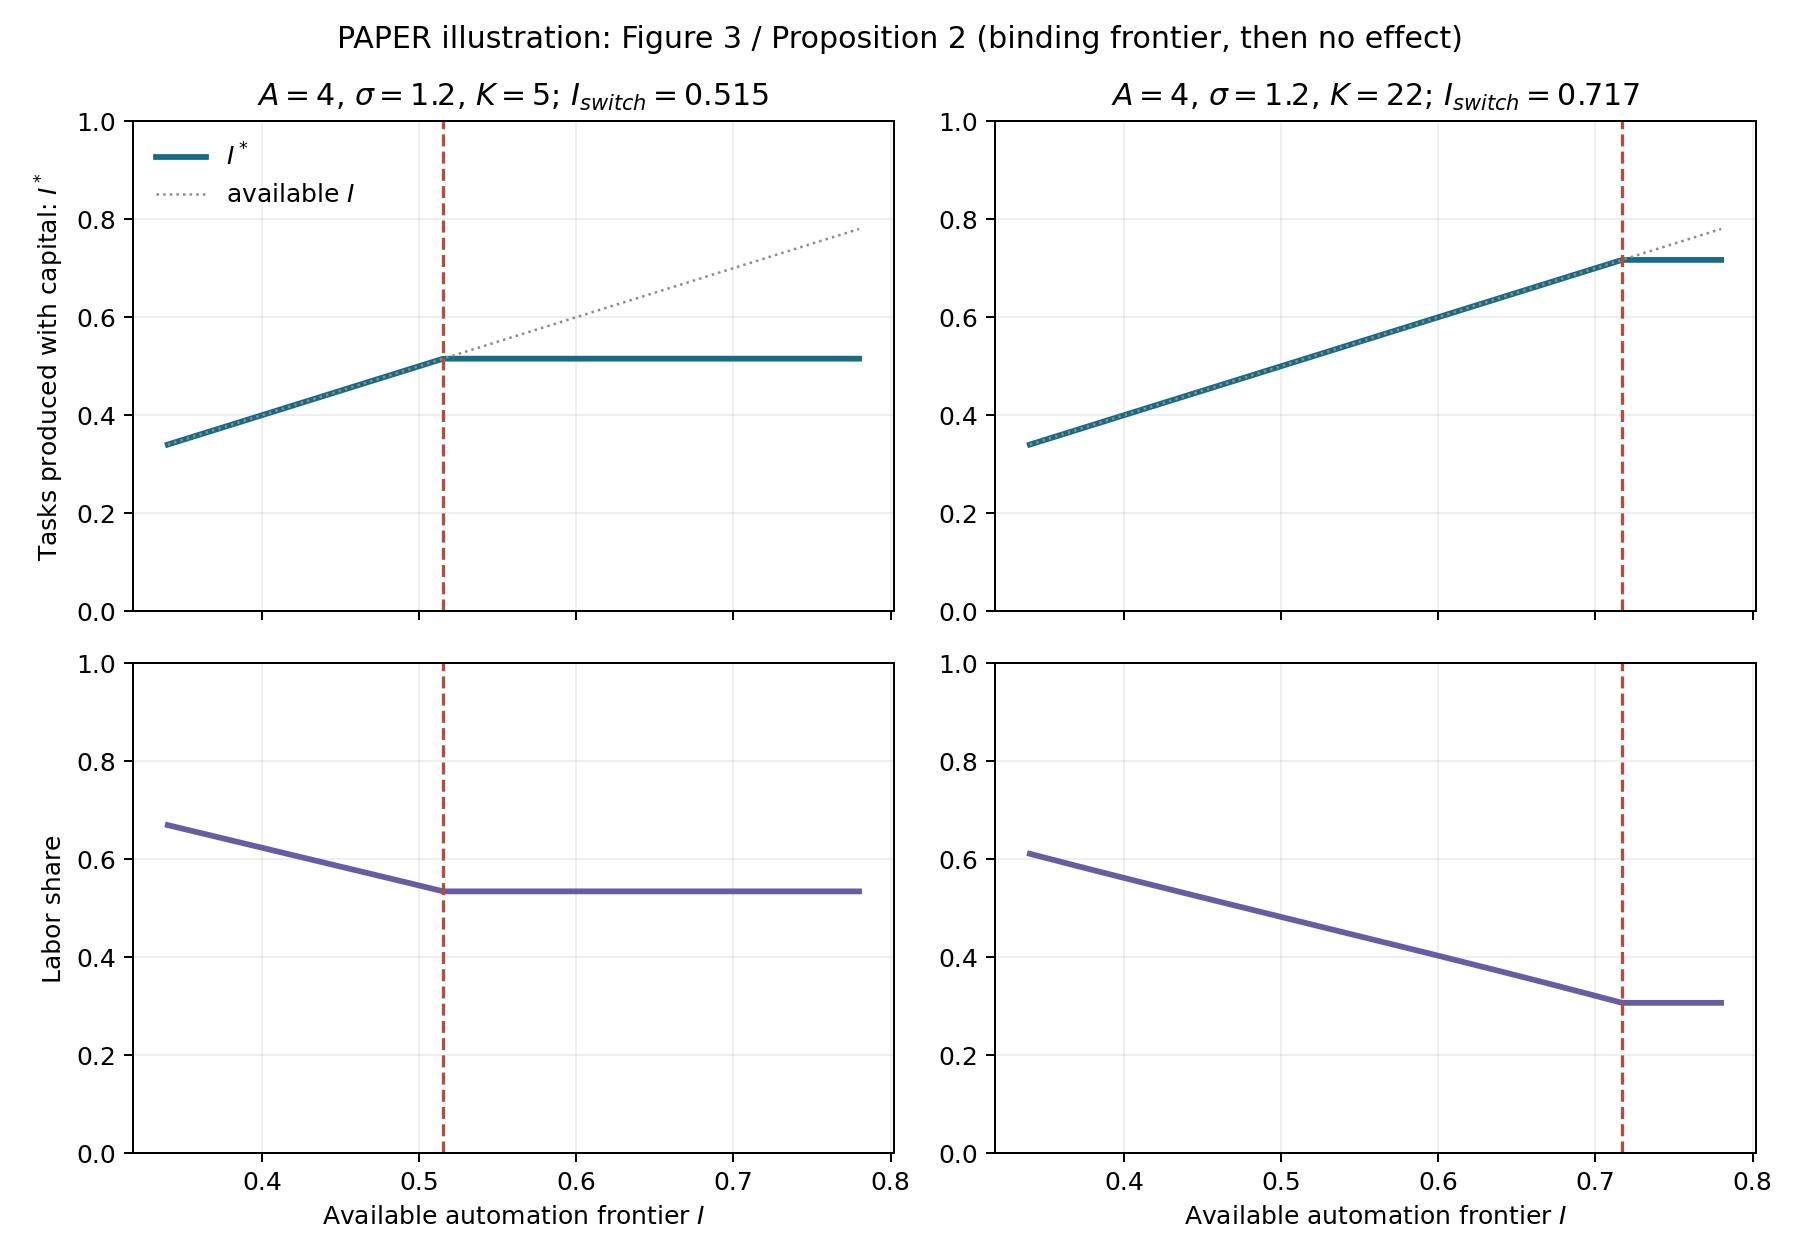
\includegraphics[width=\linewidth,height=0.70\textheight,keepaspectratio]{figures/task_allocation.png}
    \column{0.31\textwidth}
      \small
      \textbf{Paper result illustrated}

      The realized cutoff follows $I$ while automation binds. Once the
      cost-equality threshold binds, extra available automation leaves the
      allocation unchanged.

      \medskip
      The lower panels show the corresponding labor-share response.
  \end{columns}
  \source{Numerical illustration of Proposition 2 and Figure 3; generated by \texttt{sim.py}.}
\end{frame}

\begin{frame}{Numerical check: the wage threshold}
  \begin{columns}[T,onlytextwidth]
    \column{0.66\textwidth}
      \centering
      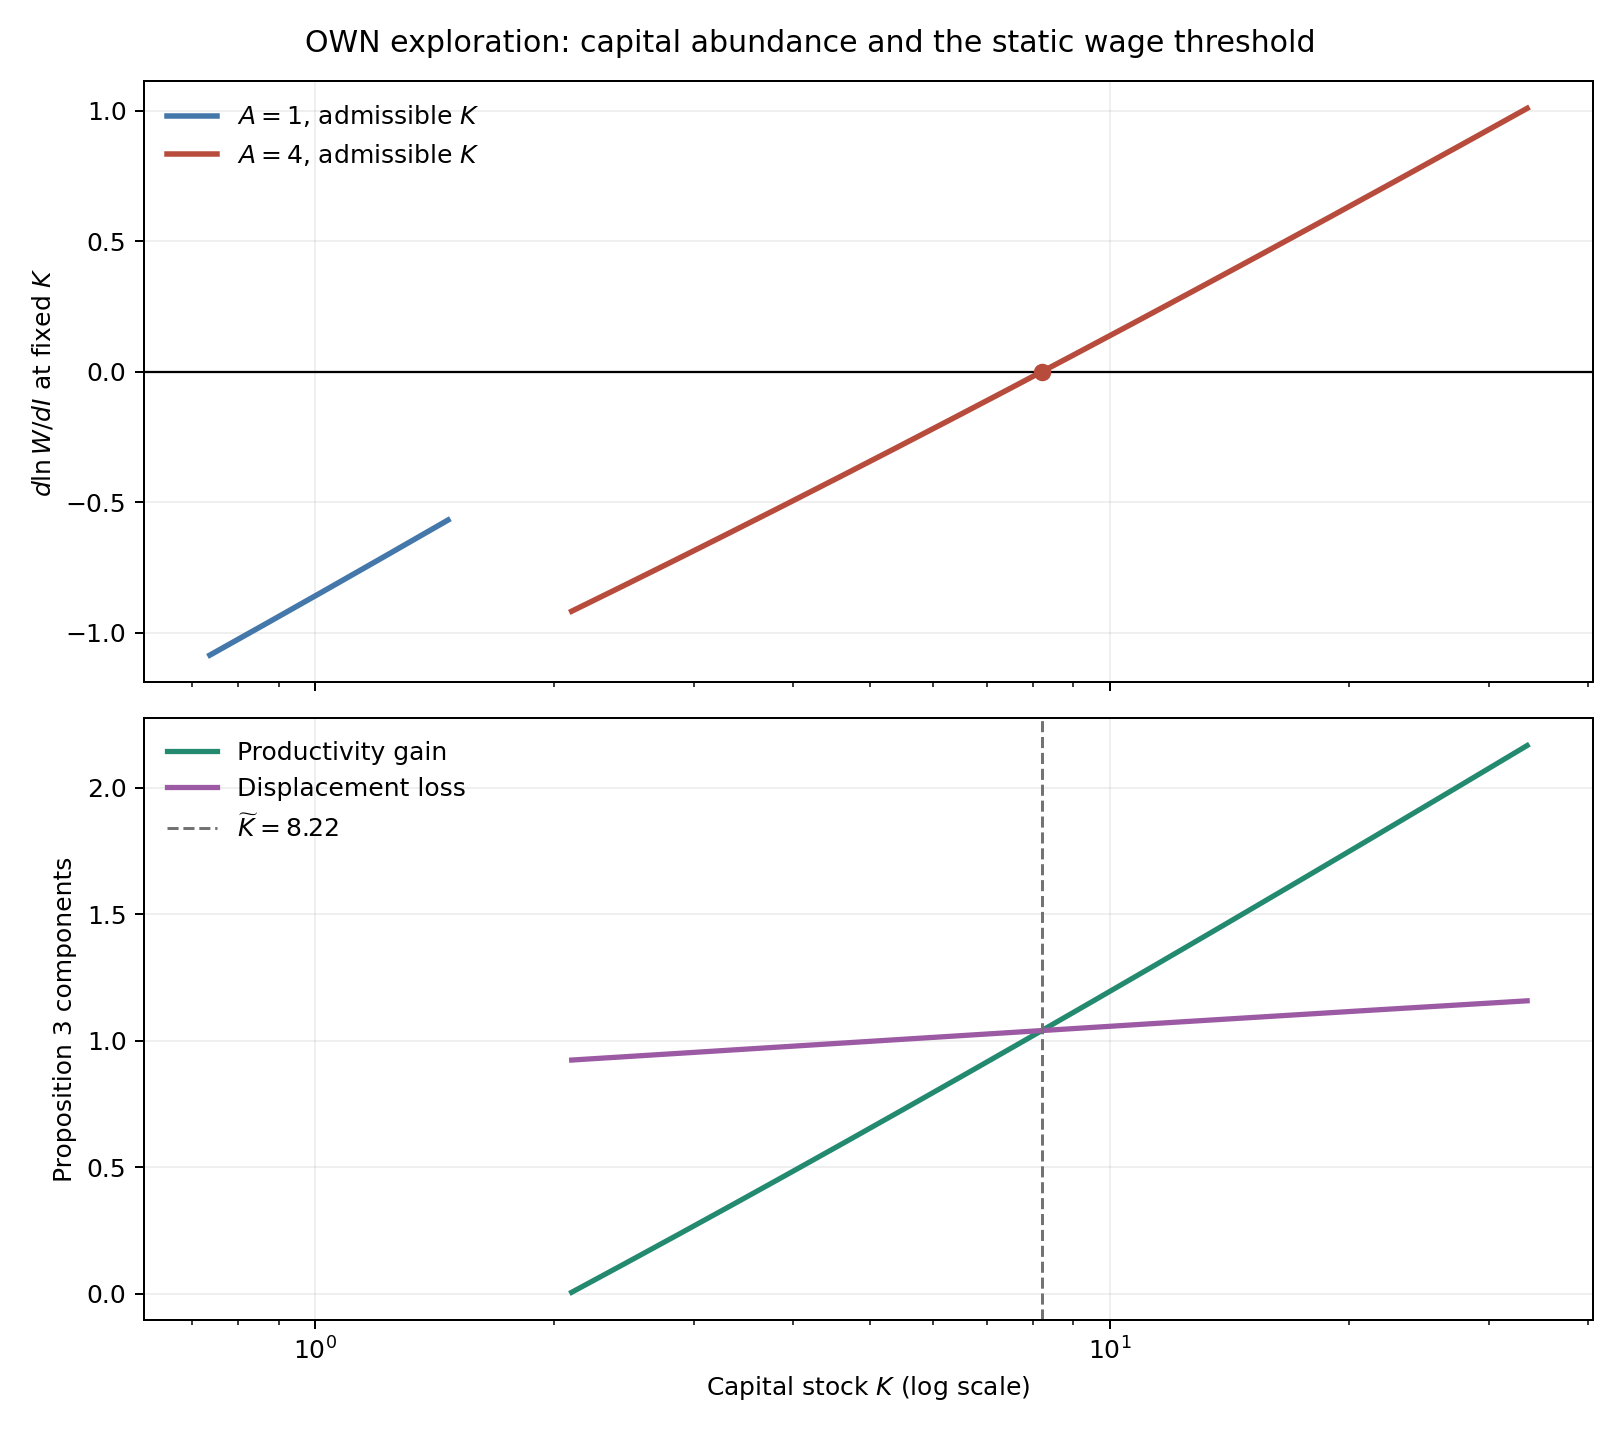
\includegraphics[width=\linewidth,height=0.70\textheight,keepaspectratio]{figures/wage_threshold.png}
    \column{0.31\textwidth}
      \small
      \textbf{Own exploration}

      The fixed-capital wage derivative changes sign when the productivity
      gain overtakes the displacement term.

      \medskip
      The analytical derivative agrees with a centered finite difference in
      the simulation.
  \end{columns}
  \source{Original numerical exploration based on the static CES model; generated by \texttt{sim.py}.}
\end{frame}

\begin{frame}{Hand check of the AI-generated derivation}
  \begin{columns}[T,onlytextwidth]
    \column{0.56\textwidth}
      \small
      Appendix B supplies
      \begin{align*}
        s_L\,d\ln W+(1-s_L)d\ln R &= d\ln Y\vert_{K,L}, &&\text{(B9)}\\
        d\ln W-d\ln R &= q. &&\text{(B10)}
      \end{align*}
      Adding $(1-s_L)$ times (B10) to (B9) isolates the wage:
      \[
        d\ln W=d\ln Y\vert_{K,L}+(1-s_L)q.
      \]
      Subtracting $s_L$ times (B10) isolates the rental rate:
      \[
        d\ln R=d\ln Y\vert_{K,L}-s_Lq.
      \]
      For automation, $q=-D$ with $D>0$, so the wage equals productivity
      minus displacement.
    \column{0.41\textwidth}
      \IfFileExists{hand/derivation.jpg}{%
        \centering\includegraphics[width=\linewidth,height=0.69\textheight,keepaspectratio]{hand/derivation.jpg}
      }{%
        \begin{block}{Photo to insert}
          Place the handwritten check at
          \texttt{hand/derivation.jpg}. The slide will include it automatically.
        \end{block}
        \medskip
        \textbf{Verdict on the AI output.} The algebra is correct. It establishes the sign
        decomposition conditional on (B9) and (B10). It does not derive those
        identities from the continuum model.
      }
  \end{columns}
  \source{NBER Appendix B, equations (B9)--(B10).}
\end{frame}

\begin{frame}{Lean formalization architecture}
  \small
  \begin{enumerate}
    \item \textbf{Source authority.} NBER Working Paper 22252, revised June 2017, pinned by SHA-256.
    \item \textbf{Model declarations.} \texttt{Assumptions.lean} defines comparative advantage, productivity positivity, automation availability, and the cost threshold.
    \item \textbf{Transparent targets.} \texttt{PaperInterface.lean} exposes two source-facing propositions as \texttt{Prop} values.
    \item \textbf{Proofs.} \texttt{MainTheorems.lean} proves the cutoff and the Proposition 3 algebra. \texttt{ProofInterface.lean} supplies exact-type endpoints.
    \item \textbf{Audit trail.} The source map records every named result and marks all unformalized results as deferred.
  \end{enumerate}

  \begin{block}{Current scope}
    The run is partially formalized. It proves two selected static results and
    records the remaining theory as proof debt.
  \end{block}
\end{frame}

\begin{frame}[fragile]{Lean result 1: the static task threshold}
  \small
  \textbf{Mathematical claim}
  \[
    I^*=\min\{I,\widetilde I\},\qquad
    i<I^* \Rightarrow R<\frac{W}{\gamma(i)}.
  \]

  \textbf{Lean statement and proof step}
  \begin{lstlisting}[style=lean]
theorem staticTaskThreshold_impl ... :
  (forall task, task < EquilibriumTaskThreshold I threshold ->
    AutomationAvailable I task /\ rental < wage / productivity task) /\ ... := by
  have hProductivity : productivity task < productivity threshold :=
    hComparativeAdvantage htaskThreshold
  rw [hThreshold] at hProductivity
  have hBeforeCleared : productivity task * rental < wage :=
    (lt_div_iff0 hRentalPositive).mp hProductivity
  \end{lstlisting}

  \textbf{Interpretation.} Strict monotonicity orders task productivity. Equation
  (6) replaces $\gamma(\widetilde I)$ by $W/R$. Positivity lets Lean clear the
  denominators without reversing the inequality.

  \source{\texttt{lean/MainTheorems.lean}, theorem \texttt{staticTaskThreshold\_impl}.}
\end{frame}

\begin{frame}[fragile]{Lean result 2: Proposition 3 algebra}
  \small
  \textbf{1. Original equations}
  \[
    s_Lw+(1-s_L)r=p,\qquad w-r=q.
  \]

  \textbf{2. Lean statement and proof fragment}
  \begin{lstlisting}[style=lean]
theorem factorPriceDecomposition_impl ...
    (hIncome : s*w + (1-s)*r = p)
    (hRelative : w-r = q) :
    w = p + (1-s)*q /\ r = p - s*q := by
  constructor
  · linear_combination hIncome + (1-s) * hRelative
  · linear_combination hIncome - s * hRelative
  \end{lstlisting}

  \textbf{3. What Lean verifies}
  \begin{itemize}
    \item All variables live in $\mathbb{R}$ and both equations are explicit hypotheses.
    \item Each proof line records the exact elimination used in the hand derivation.
    \item Lean verifies the algebra. It does not yet derive (B9) or (B10) from the production model.
  \end{itemize}

  \source{\texttt{lean/MainTheorems.lean}; GitHub Actions run 35851458024.}
\end{frame}

\begin{frame}{Verified results and open boundary}
  \begin{columns}[T,onlytextwidth]
    \column{0.48\textwidth}
      \textbf{Lean verifies}
      \begin{itemize}\small
        \item The static task threshold and both cost comparisons.
        \item The factor-price formulas implied by (B9) and (B10).
        \item The automation sign split: rental rate positive; wage sign set by productivity versus displacement.
        \item Zero \texttt{sorry}, \texttt{admit}, or added axioms.
      \end{itemize}
    \column{0.48\textwidth}
      \textbf{Still open}
      \begin{itemize}\small
        \item Derivation of (B9) and (B10) from the continuum model.
        \item Exact CES coefficient positivity.
        \item Propositions 1--2 and the dynamic results.
        \item Independent semantic closeout for every named result.
      \end{itemize}
  \end{columns}

  \begin{block}{Recorded check}
    \texttt{lake build +AR18RaceManMachine}: 8,317 jobs passed.\\
    \texttt{paper\_contribution.py check AR18RaceManMachine --fast}: passed.
  \end{block}
\end{frame}

\begin{frame}{The NBER capital-threshold clause remains unresolved}
  \small
  The pinned NBER Proposition 3 prints
  \[
    \bar K>\underline K,
  \]
  while Assumption 3 imposes $K<\underline K$. The same proposition assigns a
  negative wage effect to $K>\bar K$.

  \medskip
  Inside Assumption 3, the stated negative-wage region cannot occur. The later
  AER version reverses the economic threshold, but the Lean run uses the NBER
  paper as its source authority.

  \begin{block}{Formalization decision}
    The run records this as \texttt{AR18-P3-CAPITAL-THRESHOLD-01}. It does not
    silently substitute the AER wording or claim a complete proof of Proposition 3.
  \end{block}

  \source{NBER page 13 and Assumption 3; AER Proposition 3 used only for comparison.}
\end{frame}

\begin{frame}{Conclusion}
  \Large
  Automation does not have one uniform effect on labor.

  \medskip
  \normalsize
  \begin{itemize}
    \item The fixed-capital wage reflects productivity minus displacement.
    \item Capital adjustment can reverse the long-run wage response while employment and labor share remain lower.
    \item Lean confirms the cutoff logic and the factor-price algebra, and exposes the assumptions that the current proof still accepts rather than derives.
  \end{itemize}

  \medskip
  \textbf{Main lesson.} Formal verification sharpens the economic claim only
  when the source equation, added assumptions, and proof boundary remain visible.

  \source{Repository: \href{https://github.com/fgalarzac/ai-06-restrepo}{github.com/fgalarzac/ai-06-restrepo}.}
\end{frame}

\end{document}

